\documentclass{standalone}

\usepackage{tikzbricks}

\usepackage{tikz-3dplot}

\begin{document}


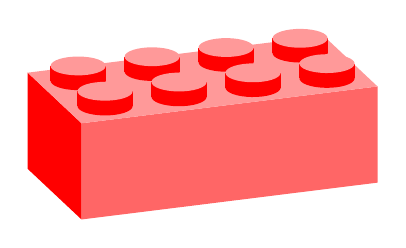
\begin{tikzpicture}
\brick{4}{2}
\end{tikzpicture}


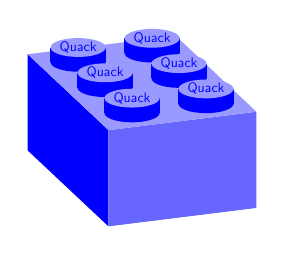
\begin{tikzpicture}
\brick[color=blue,studtext={Quack}]{2}{3}
\end{tikzpicture}


\begin{tikzpicture}
\brick[color=orange]{1}{1}
\end{tikzpicture}

\tdplotsetmaincoords{70}{110}
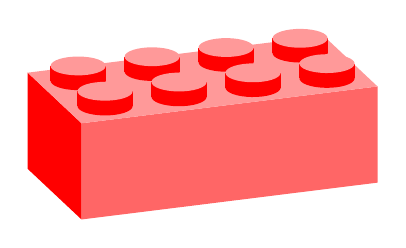
\begin{tikzpicture}
\brick{4}{2}
\end{tikzpicture}


\begin{tikzpicture}
\brick[color=teal,scale=3]{1}{1}
\end{tikzpicture}

\tdplotsetmaincoords{70}{160}
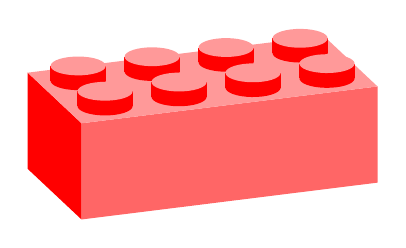
\begin{tikzpicture}
\brick{4}{2}
\end{tikzpicture}

\tdplotsetmaincoords{70}{180}
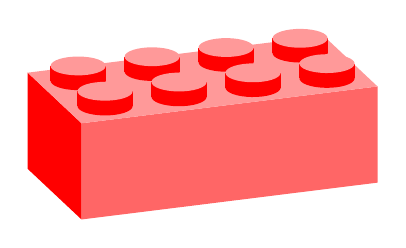
\begin{tikzpicture}
\brick{4}{2}
\end{tikzpicture}


\begin{tikzpicture}
\brick[color=teal,scale=3,studtext={TikZ}]{1}{1}
\end{tikzpicture}




\end{document}